\section{Volumetric locking: a caveat in the standard finite element method under the incompressibility constraint} 
\label{sec_volumetric_locking}

\subsection{Physical and mathematical aspects of the problem}

\subsubsection{Nearly incompressible linear elastic case}

In the linear isotropic elastic case, the material becomes
nearly-incompressible when the Poisson ratio $\nu$ tends to 0.5.
In this case, the first Lamé coefficient $\lambda$ tends to infinity.
On contrary, the second Lamé coefficient, \textit{i.e.} the shear modulus,
$\mu$ has a finite limit.

\begin{equation}
    \begin{cases}
        \begin{aligned}
            & \lambda = \frac{E\nu}{(1+\nu)(1-2\nu)}\to\infty
            \\
            & \mu = \frac{E}{2(1+\nu)}\to\frac{E}{3}
        \end{aligned}
    \end{cases}
\end{equation}

The effect of this singular behaviour of the first Lamé coefficient can be
readily be seen on the stationary Navier equation (See
\cite{shilt_solution_2020}:

\begin{equation}
    (\lambda + \mu) \nabla (\nabla \cdot \tensori{u}) + \mu \Delta \tensori{u} + \tensori{f}\subscript{V} = 0
\end{equation}

where $\tensori{u}$ is the displacement field, $\tensori{f}\subscript{V}$ the
volumetric forcing vector.

This equation can be decomposed into a regular part, proportional to
$\mu$ and a non regular part proportional to $\lambda$.

In near-incompressible cases, $\lambda$ acts as a penalisation terms
enforcing the constraint $\nabla\cdot\tensori{u} = 0$, \textit{i.e.} the
displacement must be divergence free. Equivalently, the trace of the
strain must be null, i.e. which means no change of volume (in the small
strain approximation).

\subsubsection{Non linear case}

The issue of volumetric locking was discussed in the small strain
approximation but can be extended to large strains. In large strains,
the elastoplastic law imposes a nearly-incompressible behaviour so that
$\Det(\tensorii{F})=1$ where $\tensorii{F}$ is the deformation gradient.

With finite standard elements, if the displacement (nodal variable) is
interpolated with linear or quadratic shape functions the solution space
is too weak to exactly describe the nearly-incompressibility case.

This appears with high pressure oscillations in the elements. The following 
illustration of the problem is inspired by \cite{2016_ZHANG_These}. The 
issue is illustrated in \figref{fig_locking}

\begin{figure}[h!]
    \centering
    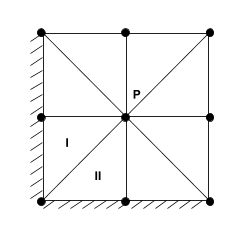
\includegraphics[width=7.cm]{img/illustrationlocking.png}
    \caption{Elements undergoing locking}
    \label{fig_locking}
\end{figure}

The material being incompressible implies that the surface of each
element has to remain constant. Consequently, the point P can only
travel vertically in the element I and move horizontally in the element
II, requiring the point to remain still. In that case, the equilibrium
equation could be not met, hence oscillations appear on the stress
field.

\subsection{Examples}

The example presented in this section are based on the internship of
Léna Moreau who reproduced some tests found in the literature with
\texttt{Cast3M} \footnotemark[1].

\footnotetext[1]{
    The \texttt{Cast3M} source files of those tests can be grabbed in the
    following git repository:
    \url{https://www-git-cad.intra.cea.fr/DEC/collaboratif/th202608/stagelenamoreau.git}
}

The first test has been extracted from \cite{2016_ZHANG_These} and
describes a hollow ball subjected to an inner pressure. Oscillations in
the pressure visualised at the integration points are clearly visible in
\figref{fig_hollow_ball} for linear and quadratic bricks.

% ![Hydrostatic pressure value field on the hollow ball meshed with linear brick (left) and quadratic brick (right)](img/HB-cub8-cu20.png){#fig:hho:hollow_ball width=90%}

\begin{figure}[h!]
    \centering
    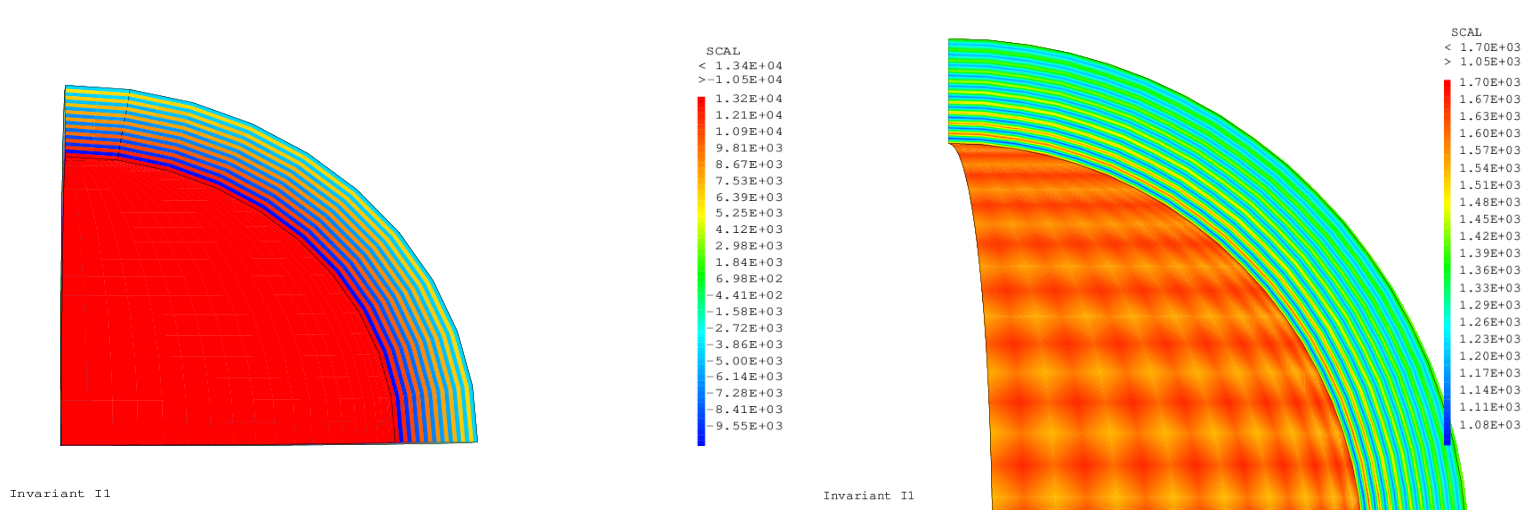
\includegraphics[width=7.cm]{img/HB-cub8-cu20.png}
    \caption{Hydrostatic pressure value field on the hollow ball meshed with linear brick (left) and quadratic brick (right)}
    \label{fig_hollow_ball}
\end{figure}

The second tests describes a cylinder is submitted to compression and
shear (controlled buckling) It is inspired by \cite{abbas_hybrid_2018}.
Again, strong oscillations of be pressure field can be observed on
\figref{fig_cylinder_test}. Usage of $\bar{B}$ elements may
alleviate the problem but only partially.

\begin{figure}[h!]
    \centering
    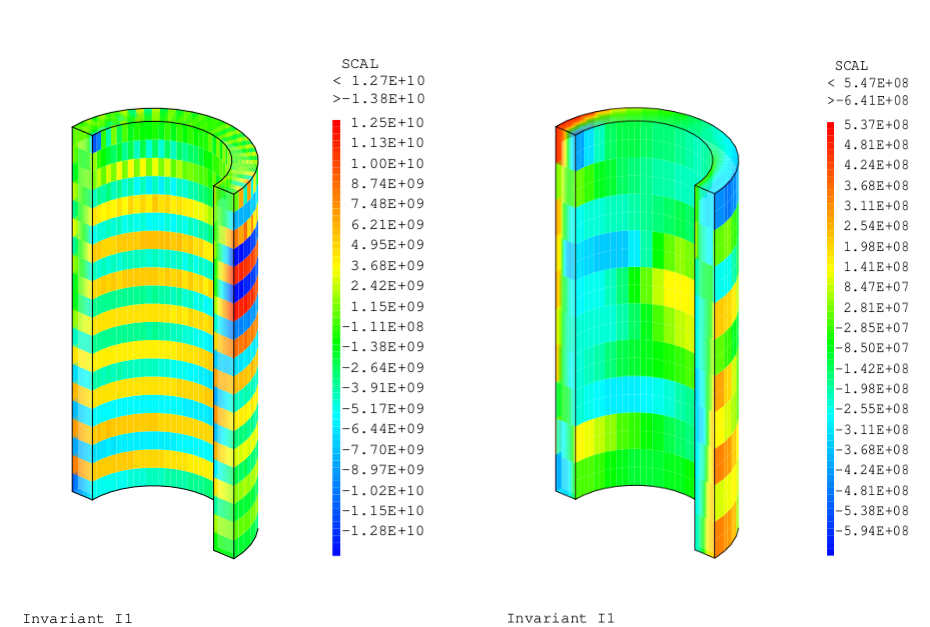
\includegraphics[width=7.cm]{img/Cylinder-cu-bbar.png}
    \caption{Hydrostatic pressure value field on the cylinder meshed with linear bricks (left) and $\bar{B}$ elements (right)}
    \label{fig_cylinder_test}
\end{figure}